% !TEX program = pdflatex
\documentclass[9pt,twocolumn]{extarticle}

\usepackage[letterpaper,top=0.66in,bottom=0.70in,left=0.66in,right=0.66in,columnsep=0.25in]{geometry}
\usepackage[T1]{fontenc}
\usepackage{lmodern}
\usepackage{microtype}
\usepackage{amsmath,amssymb}
\usepackage{booktabs}
\usepackage{tabularx}
\usepackage{array}
\usepackage{graphicx}
\usepackage{xcolor}
\usepackage{enumitem}
\usepackage{caption}
\usepackage{hyperref}
\usepackage{xurl}
\usepackage{seqsplit}

\definecolor{ink}{HTML}{17212B}
\definecolor{muted}{HTML}{5C6977}
\definecolor{ruleblue}{HTML}{285A84}
\definecolor{softblue}{HTML}{DCEAF4}
\definecolor{accent}{HTML}{B85C35}
\hypersetup{
  colorlinks=true,
  linkcolor=ruleblue,
  citecolor=ruleblue,
  urlcolor=ruleblue,
  pdfborder={0 0 0},
  pdftitle={Evaluating History-Aware Design Skills for Coding Agents},
  pdfauthor={Memi Research and Design Engineering},
  pdfsubject={Preregistered matched-pair evaluation of Memi 2.7.3}
}
\urlstyle{same}
\captionsetup{font=small,labelfont=bf,labelsep=period}
\setlength{\parindent}{1em}
\setlength{\parskip}{0pt}
\setlist{leftmargin=*,topsep=3pt,itemsep=1pt,parsep=0pt}
\setlength{\tabcolsep}{4pt}
\renewcommand{\arraystretch}{1.10}
\emergencystretch=2em
\raggedbottom

\newcommand{\Memi}{Memi}
\newcommand{\Candidate}{\texttt{@memi-design/cli@2.7.3}}
\newcommand{\Release}{\texttt{2.7.4}}
\newcommand{\sha}[1]{\texttt{\seqsplit{#1}}}
\newcommand{\artifact}[1]{\path{#1}}
\newcommand{\RQ}[1]{\textbf{RQ#1}}

% Compile-safe interface between the frozen paper and generated analysis output.
% The analysis pipeline may provide generated/tex/report-macros.tex and the
% section/figure interpretation fragments named below. Missing artifacts remain
% conspicuous and do not silently become affirmative claims.

\newcommand{\PendingArtifact}[1]{%
  \begin{center}
    \fbox{\begin{minipage}{0.92\linewidth}
      \small\textbf{Pending generated artifact.} #1
    \end{minipage}}
  \end{center}%
}

\newcommand{\InputOrPending}[2]{%
  \IfFileExists{#1}{\input{#1}}{\PendingArtifact{#2 (expected at \path{#1}).}}%
}

\newcommand{\AuditStatusLabel}{INCOMPLETE --- GENERATED RESULTS NOT LOADED}
\newcommand{\ClaimDecision}{No confirmatory quality, efficiency, or superiority
claim is authorized while generated analysis artifacts are absent.}
\newcommand{\FreshCellStatus}{Pending receipt-ledger validation.}
\newcommand{\PrimaryGateStatus}{Pending blinded grading and executed analysis.}
\newcommand{\ReleaseGateStatus}{PENDING LIVE VERIFICATION --- Memi 2.7.4
publication and public-channel parity are not established.}

\IfFileExists{generated/tex/report-macros.tex}{%
  % Generated deterministically from the executed V15 analysis; do not edit.
\renewcommand{\AuditStatusLabel}{V15 CONFIRMATORY ANALYSIS EXECUTED}
\renewcommand{\FreshCellStatus}{36 of 36 frozen cells have unique, manifest-verified receipts; no missing cell is imputed.}
\renewcommand{\PrimaryGateStatus}{Quality non-inferiority passed for buzzr-tab-unread-badge, paraform-command-menu.}
\renewcommand{\ClaimDecision}{Quality non-inferiority passed for buzzr-tab-unread-badge, paraform-command-menu. No superiority or dollar-savings claim is authorized.}
%
}{}

% Analysis output may authorize only study claims. Release authorization is a
% separate live-evidence gate and therefore remains fail-closed here.
\renewcommand{\ReleaseGateStatus}{PENDING LIVE VERIFICATION --- Memi 2.7.4
publication and public-channel parity are not established.}

\newcommand{\FigurePlaceholder}[1]{%
  \fbox{\begin{minipage}[c][43mm][c]{0.94\linewidth}
    \centering\small\textbf{Pending generated figure}\par\medskip
    #1
  \end{minipage}}%
}

\newcommand{\QualityFigure}{%
  \IfFileExists{generated/figures/paired_quality_comparisons.png}{%
    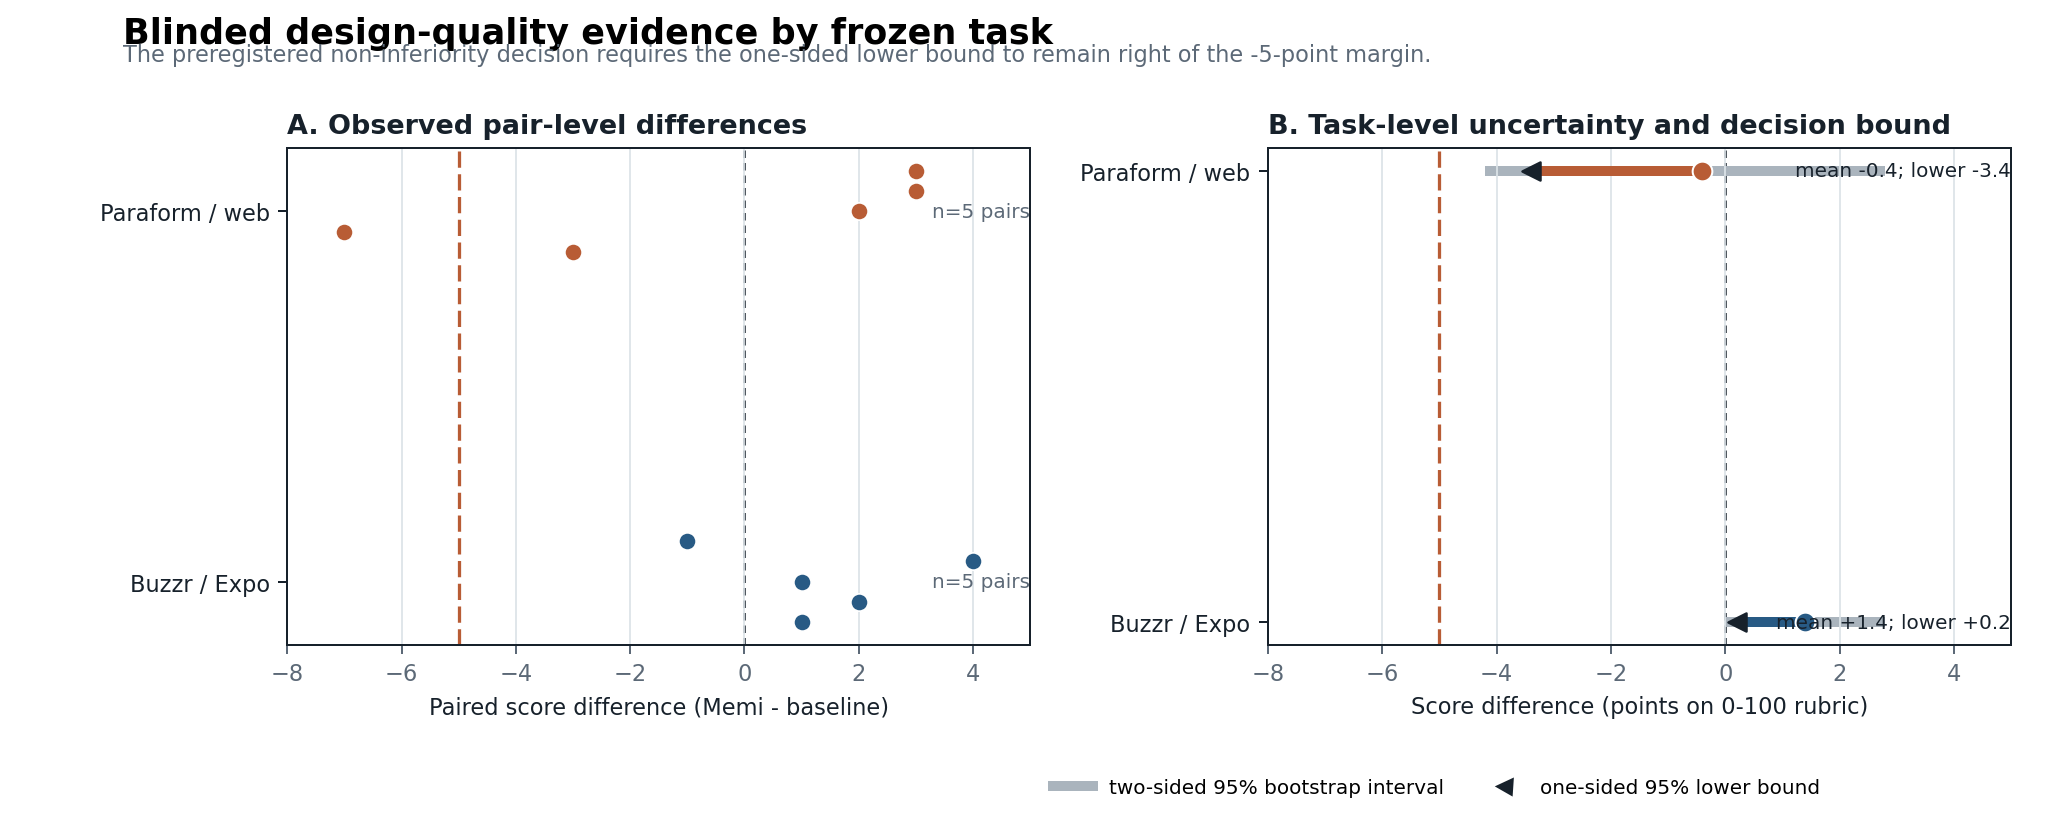
\includegraphics[width=\linewidth]{generated/figures/paired_quality_comparisons.png}%
  }{\IfFileExists{generated/figures/primary_task_mean_deltas.png}{%
    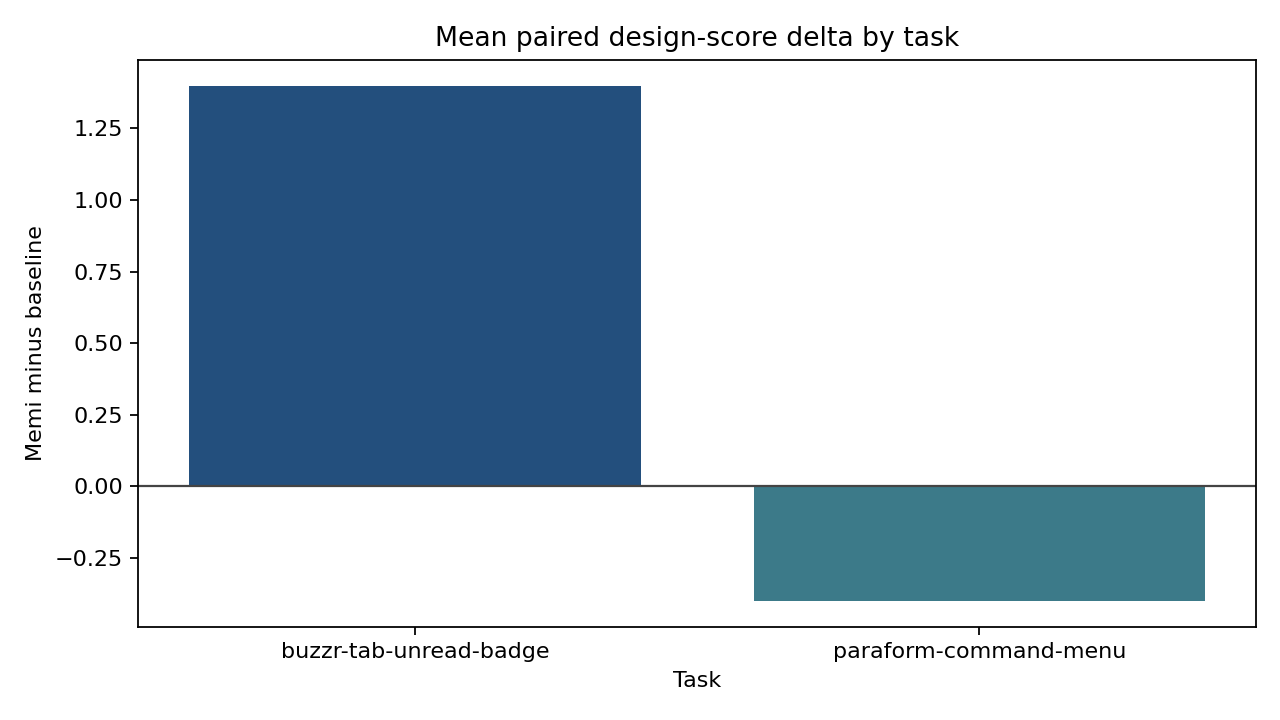
\includegraphics[width=\linewidth]{generated/figures/primary_task_mean_deltas.png}%
  }{\FigurePlaceholder{Paired quality comparisons by task.}}}%
}

\newcommand{\ResourceFigure}{%
  \IfFileExists{generated/figures/task_resource_intervals.png}{%
    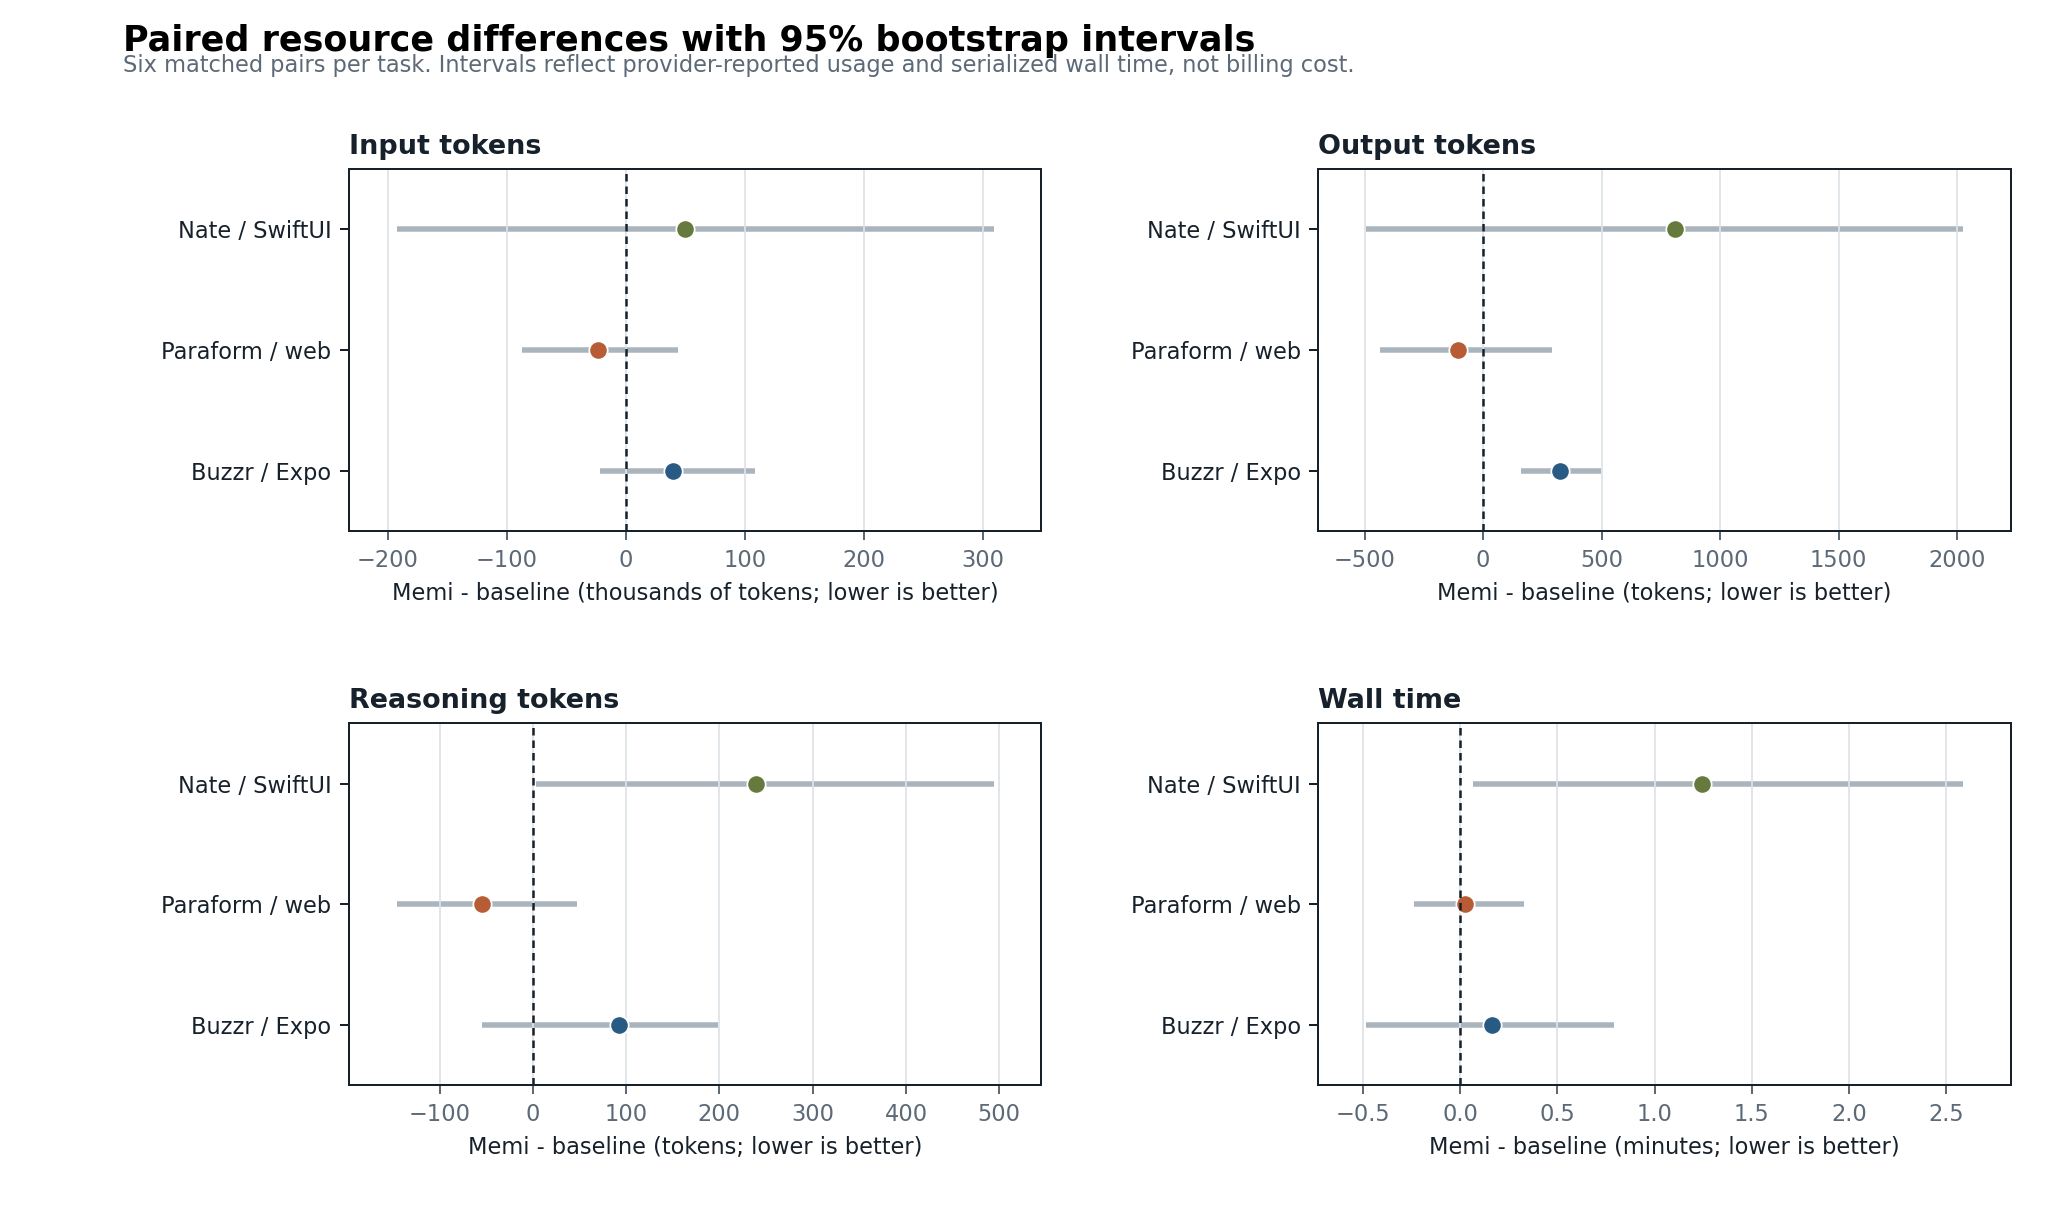
\includegraphics[width=\linewidth]{generated/figures/task_resource_intervals.png}%
  }{\FigurePlaceholder{Task-faceted paired resource intervals.}}%
}

\newcommand{\BacktestFigure}{%
  \IfFileExists{generated/figures/fitness_backtest.png}{%
    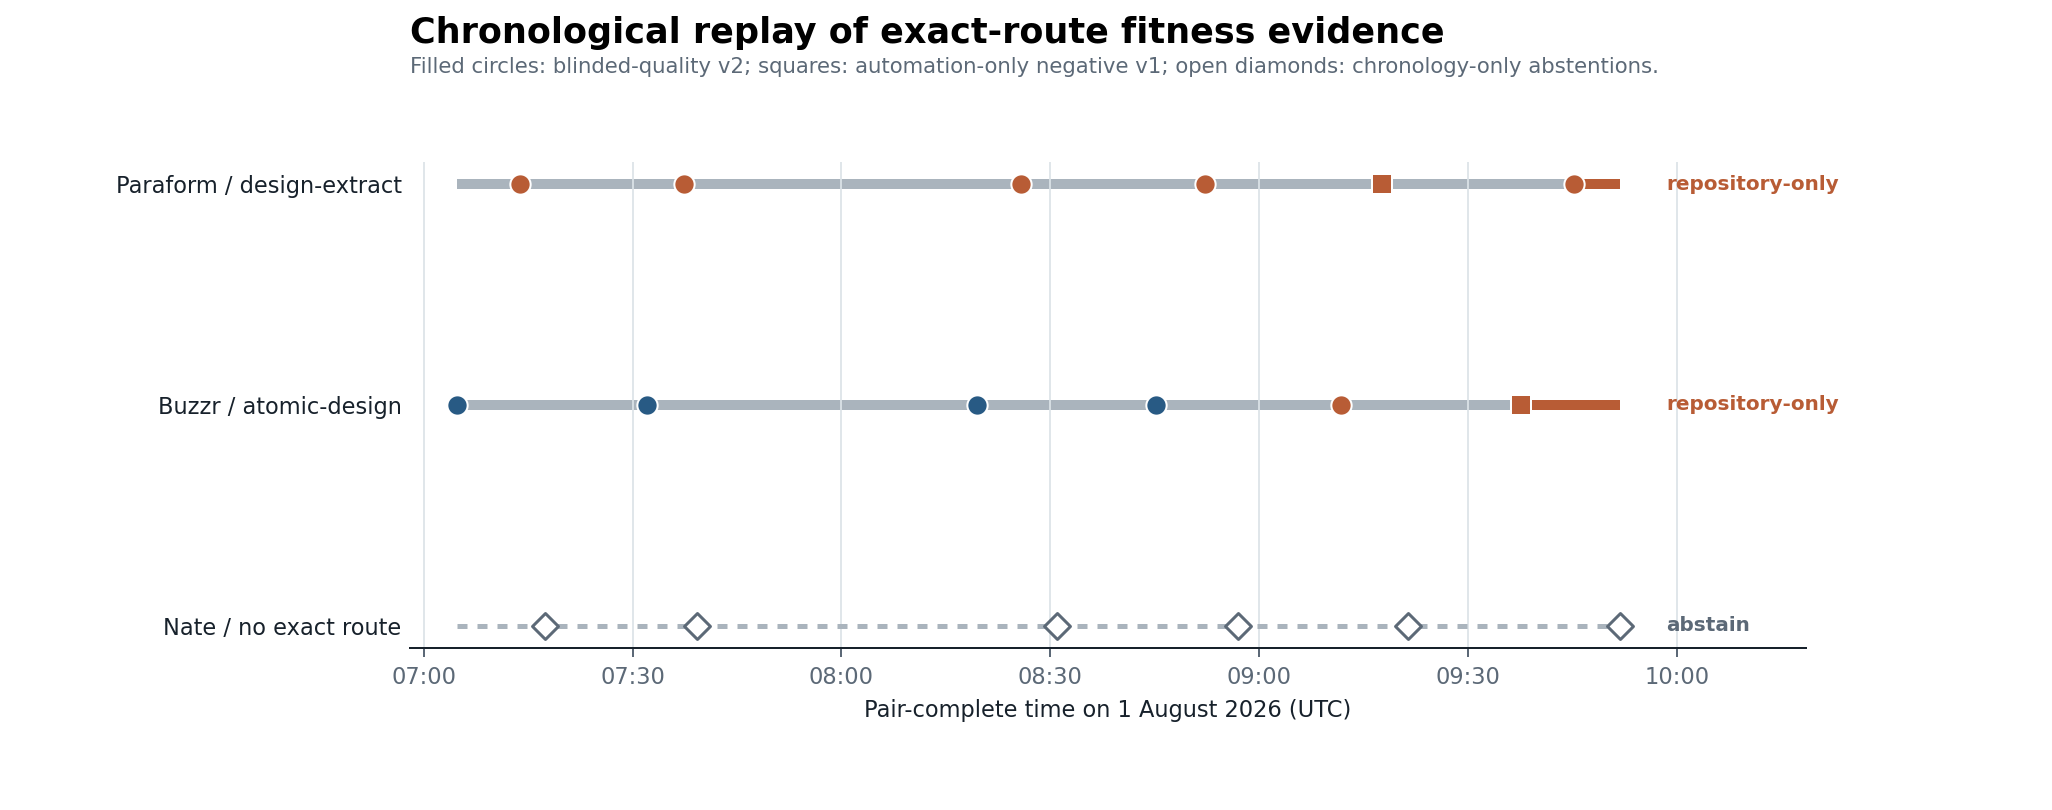
\includegraphics[width=\linewidth]{generated/figures/fitness_backtest.png}%
  }{\IfFileExists{generated/figures/chronological_fitness_backtest.png}{%
    \includegraphics[width=\linewidth]{generated/figures/chronological_fitness_backtest.png}%
  }{\FigurePlaceholder{Chronological, no-look-ahead routing-policy replay.}}}%
}


\title{\vspace{-1.2em}\textbf{Evaluating History-Aware Design Skills for Coding Agents:}\\[0.2em]
\large A Preregistered Matched-Pair Study of Memi 2.7.3}
\author{Memi Research and Design Engineering\\
\small Public technical disclosure and reproducibility report}
\date{1 August 2026}

\begin{document}
\color{ink}
\twocolumn[\maketitle\vspace{-1.5em}]

\begin{abstract}
Coding agents can receive repository-specific design skills, but successful
automation does not establish that the resulting interface is usable, that a
skill transfers safely to a new repository, or that historical success should
authorize future use. We evaluate the exact published Memi 2.7.3 artifact in a
preregistered matched-pair study spanning web, Expo, and SwiftUI repositories.
Thirty-six serialized agent cells formed 18 baseline/Memi pairs under the same
provider, model, effort, task contract, and verification rules. All 36 receipts
passed content-addressed admission. Fourteen cells were excluded only from
rendered grading, leaving 10 complete quality pairs across two tasks. Three
blinded model graders scored a 100-point interface rubric. The mean
Memi-minus-baseline score difference was $+1.4$ for Buzzr (one-sided 95\%
lower bound $+0.2$) and $-0.4$ for Paraform (lower bound $-3.4$); both bounds
exceeded the preregistered $-5$ point non-inferiority margin. Neither task
established superiority, and no quality estimate was possible for Nate. Across
21 task-by-resource tests, no comparison remained significant after Holm
correction. The evidence motivated a fail-closed router released in Memi 2.7.4:
history is isolated by exact task, repository, harness, skill identity, and
skill-content hash; a harmful event suppresses immediately; recovery requires
three later healthy prospective pairs. A chronological replay left both
observed routes suppressed and repository-only. We release the executed
notebook, receipts, exclusions, grader records, figures, policy replay, and
software-channel provenance. The findings are model-graded product research,
not independent practitioner validation.
\end{abstract}

\noindent\textbf{Keywords:} coding agents; design engineering; matched-pair
evaluation; non-inferiority; LLM-as-a-judge; evidence-based routing;
reproducible systems research

\section{Introduction}

Repository-level coding benchmarks have made execution in real codebases a
central unit of evaluation \cite{jimenez2024swebench}. Interactive-agent work
similarly emphasizes outcome-based validation in realistic environments
\cite{zhou2024webarena}. Frontend engineering adds a second problem: a patch
may compile and pass a functional test while still degrading accessibility,
hierarchy, responsiveness, or design-system consistency. Design-to-code
benchmarks have documented the distance between visual generation and robust
frontend implementation \cite{si2024design2code}, but less is known about
agents that receive reusable design instructions inside an existing codebase.

Memi is a design-skill and audit layer for coding agents. Its router can select
repository-relevant skill content before an agent edits code. This creates a
deployment question that is both statistical and operational: when does past
evidence justify enabling a skill route, and what should happen after a quality
or efficiency regression? A permissive history mechanism can leak evidence
across repositories, models, or revised skill content. A purely functional
benchmark can miss interface regressions. A release checklist can verify
distribution without answering either research question.

This paper reports V15, a prospective confirmatory study of the exact Memi
2.7.3 npm artifact, and the fail-closed policy that followed in 2.7.4. It asks:

\begin{enumerate}[label=\textbf{RQ\arabic*:},leftmargin=*,labelsep=0.5em]
  \item \textbf{Interface quality.} Within each frozen task with complete
  rendered evidence, is Memi's model-graded design quality non-inferior to the
  baseline agent under a $-5$ point margin?
  \item \textbf{Function and resources.} How do functional acceptance,
  critical defects, token use, wall time, tool calls, retries, and provider
  failures differ within matched pairs?
  \item \textbf{Safe reuse.} Can exact-route historical evidence be replayed
  without look-ahead and converted into a policy that suppresses harmful routes
  without borrowing evidence from another task, repository, model, or skill
  revision?
\end{enumerate}

The contributions are: (i) a preregistered, multi-platform matched-pair study;
(ii) an evidence model that separates execution validity, functionality,
renderability, and blinded quality; (iii) a chronological backtest of an
exact-match, fail-closed router; and (iv) a public artifact package that binds
the analysis to published software channels. The paper makes no general
superiority or dollar-savings claim.

\section{Related work and positioning}

\textbf{Repository-level agent evaluation.} SWE-bench evaluates patches against
real repository tests, demonstrating the importance of pinned code state and
executable outcomes \cite{jimenez2024swebench}. WebArena extends realistic,
functional evaluation to interactive web tasks \cite{zhou2024webarena}. V15
adopts the same high-level principle--evaluate the produced artifact in its
repository--but adds matched conditions, interface-quality grading, content
hashes, and release provenance.

\textbf{Frontend and design evaluation.} Design2Code combines rendering-based
metrics with human evaluation and reports persistent layout and visual-element
failures in automated frontend generation \cite{si2024design2code}. V15 instead
studies bounded edits to existing products. The outcome therefore includes
task correctness, accessibility, design-system fit, responsiveness, and code
quality rather than screenshot similarity alone.

\textbf{Model-based grading.} Strong language models can approximate preference
judgments, but position, verbosity, and self-enhancement biases remain material
\cite{zheng2023judge}. We therefore blind condition labels, use three graders,
report disagreement and ICC, exclude non-renderable evidence, and describe the
result as \emph{model-graded}. We do not substitute this panel for independent
practitioner evidence.

\section{Study design}

\subsection{Candidate, conditions, and tasks}

The candidate was the immutable npm tarball for \Candidate{}, SHA-256
\sha{b2b56189f45b69a3cec41220ae3e9d50d6ecfb682aee5a64c1fe0ce0d0ec3e1e}.
The baseline condition used the provider agent under the frozen task contract
without a Memi-routed design skill. The Memi condition used the same contract
and could receive at most one routed skill, recorded in its route receipt.
Provider (Codex), model (\texttt{gpt-5.6-luna}), reasoning effort (low), maximum
input tokens (450,000), verification rules, and fixture revision were held
constant within each pair.

Three tasks were selected to exercise different interface stacks and forms of
interaction (Table~\ref{tab:tasks}). Six pairs were run per task. Condition
order was counterbalanced with frozen seed 2715. Cells executed serially; Xcode
and Simulator received exclusive machine access.

\begin{table}[t]
\centering
\caption{Frozen task strata and required behavior.}
\label{tab:tasks}
\small
\begin{tabularx}{\columnwidth}{@{}p{0.15\columnwidth}p{0.13\columnwidth}Xr@{}}
\toprule
Fixture & Stack & Required change & Pairs \\
\midrule
Buzzr & Expo & Accessible unread-count badge & 6 \\
Paraform & Web & Keyboard command menu & 6 \\
Nate & SwiftUI & Truthful reduced-motion state & 6 \\
\bottomrule
\end{tabularx}
\end{table}

\subsection{Prospective execution and evidence admission}

Each cell began from a clean clone at a pinned revision. Preparation, routing,
patch, tool activity, usage, environment, isolated verification, and final run
receipt were recorded. The admission pipeline rejected missing artifacts,
duplicate trial identities, fixture mutation, hash disagreement, condition
mismatch, or non-isolated verification. All evidence was content-addressed.

Figure~\ref{fig:design} shows the central evidence boundary. Functional and
resource outcomes use every admitted receipt. Rendered quality uses only cells
with reviewable interface evidence; a grading-only exclusion does not erase
the cell's other outcomes. This distinction prevents render failures from being
silently imputed while retaining observed execution failures as data.

\begin{figure*}[t]
\centering
\StudyDesignFigure
\caption{Prospective execution and evidence admission. All 36 cells entered
functional and resource analysis. Fourteen prespecified, cell-level exclusions
applied only to rendered grading; 22 cells were graded and 20 formed 10 complete
quality pairs.}
\label{fig:design}
\end{figure*}

\subsection{Blinded interface-quality panel}

Three model graders independently scored anonymized evidence. Condition labels
were hidden. The rubric allocated 25 points to task and interaction correctness,
20 to accessibility, 15 each to visual hierarchy, design-system consistency,
and responsive/adaptive behavior, and 10 to implementation quality. Dimension
and total scores were aggregated by panel median. We report absolute
disagreement and ICC(2,1), following the two-way random-effects reliability
formulation of Shrout and Fleiss \cite{shrout1979icc}.

The rendering boundary is important. Buzzr's evidence is a React Native testing
renderer tree rather than native pixels. Paraform has registered desktop
browser states, while its phone breakpoint intentionally replaces the desktop
workspace. All 12 Nate cells lacked admissible rendered grading evidence. These
constraints limit visual inference even when functional receipts are valid.

\subsection{Evidence lineage}

The earlier V14 study remains labeled 2.7.2 feasibility evidence: 12 cells and
six pairs across Buzzr and Paraform, without Nate or a blinded rendered panel.
It is neither relabeled nor pooled into V15. Release reconstruction found that
2.7.3 changed release metadata, guidance, and adapter-test stabilization rather
than the previously benchmarked runtime paths; V15 nevertheless executed the
exact 2.7.3 tarball instead of inferring behavior from that source comparison.

\section{Statistical analysis}

The experimental unit is a matched baseline/Memi pair within one task. For
quality, the paired estimand is
\begin{equation}
  \Delta_q = q_{\mathrm{Memi}} - q_{\mathrm{baseline}}.
\end{equation}
We report the task-level mean and median, the exact sign test, a 10,000-sample
paired bootstrap interval \cite{efron1993bootstrap}, and leave-one-pair-out
sensitivity. The preregistered affirmative rule is non-inferiority, not
superiority: the one-sided 95\% lower bound must be strictly greater than
$-5$ points on the 100-point rubric. The margin was frozen before execution.

Secondary outcomes are functional acceptance, critical defects, provider-
reported input/output/reasoning tokens, wall time, tool calls, retries, and
provider failures. Raw differences are Memi minus baseline. Tests are oriented
so that higher functional acceptance and lower values elsewhere are favorable.
Holm's sequential correction is applied across task-level secondary tests
\cite{holm1979}. Because tasks differ in platform and behavior, pooled
cross-fixture results are descriptive. No token measurement is converted into
dollars because billing records were not collected.

Missing quality pairs are not imputed. A complete functional receipt remains
in secondary analysis even if rendered grading is unavailable. Critical-defect
analysis requires complete blinded/rendered evidence and therefore has a
smaller denominator. The executed notebook is the numerical source of record;
the paper imports generated tables and figure assets from that pipeline.

\section{Results}

\subsection{All cells were admitted; rendered evidence was incomplete}

All 36 frozen cells had unique, manifest-verified receipts. Fourteen exclusions
applied only to rendered grading: all 12 Nate cells, Buzzr repeat 6 Memi, and
Paraform repeat 5 baseline. Twenty-two cells received grades. Twenty formed 10
complete pairs--five Buzzr and five Paraform--while two graded cells remained
unpaired after sibling exclusion. No value was imputed.

\subsection{\RQ{1}: Quality was non-inferior on two renderable tasks}

Figure~\ref{fig:quality} separates observed pair differences from the
task-level decision statistic. Buzzr's mean difference was $+1.4$ points
(median $+1$; two-sided 95\% bootstrap interval $0.0$ to $+2.8$); its one-sided
lower bound was $+0.2$. Paraform's mean was $-0.4$ (median $+2$; interval
$-4.2$ to $+2.8$); its one-sided lower bound was $-3.4$. Both lower bounds lie
above the $-5$ margin. Exact one-sided sign-test $p$ values were 0.1875 and 0.5,
respectively; these do not establish superiority.

\begin{figure*}[t]
\centering
\QualityFigure
\caption{Blinded design-quality evidence. Panel A shows every complete pair.
Panel B shows task means, two-sided 95\% paired-bootstrap intervals, and the
one-sided lower bounds used for the preregistered non-inferiority decision.
The orange reference is the $-5$ point margin; the zero line denotes equality.}
\label{fig:quality}
\end{figure*}

\InputOrPending{generated/tex/primary-task-summary.tex}{The task-level quality
table must be generated from the executed analysis.}

The panel's pooled ICC(2,1) was 0.531536. Pair-level absolute disagreement
varied across tasks and conditions, so the median score should not be read as a
human consensus estimate. No blinded critical defect was recorded in the 10
complete graded pairs. Nate has no quality estimate; functional success cannot
fill that missing construct.

\subsection{\RQ{2}: No secondary test survived multiplicity correction}

Functional acceptance differed by $-0.1667$ for Buzzr, $0$ for Nate, and
$+0.1667$ for Paraform. All Holm-adjusted $p$ values were 1. Critical-defect
differences were zero where renderable pairs existed; Nate had no admissible
critical-defect estimate.

Figure~\ref{fig:resources} reports the four continuous resource outcomes. Four
of 21 task-by-resource bootstrap intervals excluded zero before multiplicity
correction, but none of the 21 task-level secondary tests rejected after Holm
correction. The estimates are heterogeneous: for example, Nate showed wider
token and wall-time intervals than the other tasks. The data do not support a
general efficiency claim, and provider-reported tokens are not billing cost.

\begin{figure*}[t]
\centering
\ResourceFigure
\caption{Task-level paired resource differences. Points are mean Memi-minus-
baseline differences and lines are two-sided 95\% paired-bootstrap intervals.
Each task contributes six pairs. Negative values favor lower Memi resource use;
units are shown per panel.}
\label{fig:resources}
\end{figure*}

Sparse count outcomes are retained in the machine-readable secondary table:
tool calls, retries, and provider failures. Nate's provider-failure interval
favored Memi before correction, while Buzzr had a small positive retry
difference; neither authorized a corrected claim. Serial execution controls
local contention but does not estimate concurrent throughput.

\section{Fail-closed evidence routing}

\subsection{Policy derived from exact route identity}

The 2.7.4 policy defines a route by the exact tuple
\begin{multline}
R=(\text{task class},\text{repository fingerprint},\text{provider},\\
\text{model},\text{effort},\text{skill ID},\text{skill content hash}).
\end{multline}
Evidence from another tuple is ineligible. Fitness evidence v2 binds blinded
quality data and its SHA-256 to that identity while preserving v1 loading. A v1
negative event may suppress; automation-only v1 evidence cannot promote or
recover. This asymmetry makes legacy uncertainty conservative.

Figure~\ref{fig:policy} expresses the state machine. A quality regression, or a
joint catastrophic regression of at least 50\% more tokens and 25\% more
latency, suppresses immediately. Normal execution then falls back to
repository-only discovery. Recovery is possible only through three later
healthy, prospective, exact-match v2 pairs. New harmful evidence resets
recovery progress. A route without exact evidence abstains rather than
borrowing a favorable record.

\begin{figure*}[t]
\centering
\PolicyFigure
\caption{Fail-closed skill-fitness policy. Exact identity is checked before
historical evidence can affect execution. Suppression is immediate; promotion
from legacy automation evidence is prohibited; recovery requires three later
healthy prospective pairs on the same route.}
\label{fig:policy}
\end{figure*}

\subsection{\RQ{3}: Replay suppressed both observed routes}

The chronological backtest replayed 12 store-write-eligible events in
pair-complete order: 10 blinded-quality v2 events and two automation-only
negative v1 events. Seven additional rows were chronology-only. At each cutoff,
the replay consumed only events with timestamps at or before that cutoff.

Figure~\ref{fig:backtest} shows the resulting trajectories. Paraform/
\texttt{design-extract} was suppressed by its first exact event. Buzzr/
\texttt{atomic-design} remained healthy through four events and was suppressed
at 09:11 UTC after a quality regression. Neither route accumulated three
eligible recovery pairs. Nate abstained in all six repeats; therefore no Nate
route state or suppression claim exists.

\begin{figure*}[t]
\centering
\BacktestFigure
\caption{No-look-ahead replay of observed route evidence. Marker shape denotes
evidence version or chronology-only abstention; line color denotes the state
after each event. Both instantiated routes finish suppressed with repository-
only discovery. Nate never instantiated an exact route.}
\label{fig:backtest}
\end{figure*}

The replay validates deterministic policy mechanics and temporal isolation. It
does not show that this event stream represents future repositories, models,
providers, or skill revisions.

\section{Frontend and release validation}

\subsection{Independent product-surface audit}

The public website was audited from clean checkouts, excluding deployment
metadata, build output, generated community examples, and other non-product
sources from design review. The controlled baseline reproduced a serious
Lighthouse \texttt{label-content-name-mismatch} finding in all nine reports
across three routes. A footer accessible-name correction aligned the computed
name with visible text. All nine post-fix reports contained no blocking
accessibility finding, and the unchanged Lighthouse assertion gate moved from
exit 1 to exit 0. The Chromium light-mode suite passed 55/55 tests before and
after. The selected axe rules also passed in both conditions because the
experimental Lighthouse rule was outside that frozen selection.

This before/after result supports one narrow conclusion: the observed accessible-
name defect was removed under the unchanged gate. Local performance variation
is not interpreted causally, and local Astro execution is not deployment proof.

\subsection{Release verification as disclosure, not efficacy evidence}

Memi 2.7.4 shipped the exact-route policy through trusted-publisher OIDC.
Independent channel receipts verified npm \texttt{latest}, a nine-cell Node
20/22/24 install matrix on Linux, macOS, and Windows, the GitHub tag and platform
binaries, Action \texttt{v2}, Homebrew stable, GHCR \texttt{latest}, the MCP
Registry, and the production website artifact. The public gate returned
\texttt{failures: []} and \texttt{parityEligible: true}. GHCR was verified by
an authenticated promotion workflow; anonymous pullability is not claimed.

These receipts establish that the disclosed implementation and paper were
published consistently. They are not observations in the V15 efficacy study
and do not increase its sample size.

\section{Discussion}

\textbf{\RQ{1}.} Within the two tasks that produced complete rendered pairs,
the lower confidence bounds exceeded the preregistered non-inferiority margin.
This is evidence against a quality loss larger than five rubric points under
the observed conditions. It is not evidence that Memi is superior, and it says
nothing about Nate's rendered quality.

\textbf{\RQ{2}.} Functional and resource estimates did not yield a corrected
secondary claim. Wide and task-dependent intervals are scientifically useful:
they show that one aggregate efficiency number would hide platform-specific
behavior. A future cost study must collect billing data directly.

\textbf{\RQ{3}.} Exact-route replay changed the operational decision even where
task-level non-inferiority passed. This is not contradictory. The router's
event-level quality regression rule is deliberately more conservative than the
paper's task-level mean non-inferiority statement. Research inference asks what
the observed paired sample supports; deployment policy asks whether any exact
route has accumulated enough safe prospective evidence to remain enabled.

The broader lesson is methodological: compile success, test success, rendered
quality, policy eligibility, and distribution parity are different constructs.
A credible agent-system report should preserve those boundaries instead of
turning them into one composite score.

\section{Threats to validity}

\textbf{Internal validity.} Pairing, counterbalancing, frozen fixtures, serial
execution, and isolated verification reduce known confounding. They do not
eliminate stochastic provider behavior. Two orchestration deviations are
recorded: the admission harness was separated from the exact 2.7.3 runtime, and
a stalled partial attempt was retained as retry evidence while only the later
complete receipt supplied the trial outcome.

\textbf{Construct validity.} The 100-point rubric covers important interface
dimensions but is not a validated human-preference instrument. Model graders
may share biases with the evaluated agent family. Buzzr lacks native pixel
evidence; Paraform's mobile state is intentionally a desktop-only placeholder;
Nate lacks rendered grades entirely. Functional acceptance and critical
defects use different admissible denominators.

\textbf{Statistical conclusion validity.} Quality inference uses five complete
pairs per estimable task, and secondary analyses use six. Bootstrap intervals
and leave-one-pair-out checks expose instability but cannot create power. The
$-5$ margin is a preregistered engineering tolerance, not a universally accepted
clinical or perceptual threshold. Exact sign tests and Holm correction are
conservative at this sample size.

\textbf{External validity.} The study covers three repositories, one provider/
model/effort configuration, one Apple-silicon workstation, and one day of
execution. It does not estimate multi-user throughput, maintainability,
independent practitioner preference, billing cost, or performance on
unregistered repositories.

\textbf{Researcher independence.} The study was executed and reported by the
team developing Memi. The prospective freeze, machine-readable ledgers,
condition blinding, immutable artifacts, and public negative results improve
auditability but do not replace independent replication.

\section{Reproducibility and disclosure}

The source of record is the executed \artifact{analysis.ipynb}. The public
package contains the frozen protocol and plan, environment, rubric, exact
candidate provenance, task contracts, 36 evidence receipts, exclusion and
deviation ledgers, blinded grader records, pair-level and task-level tables,
10,000-sample bootstrap results, leave-one-pair-out sensitivity, figures,
fitness-policy inputs and replay, LaTeX source, PDF, and checksum inventories.
The report builder rejects stale derived files, duplicate JSON keys,
non-finite numbers, digest mismatch, and disagreement between release channels.

The exact candidate source commit is
\sha{2e29c5c656ac34242369eac9840838619ad113e1}. The published 2.7.4
implementation is bound to
\sha{8aa4649f412bbcaaf2af4ee209bf79016566f035}. V14 remains separately labeled
and hashed. All headline numbers can be recomputed without the prose layer.

\textbf{Conflict-of-interest statement.} Memi Research and Design Engineering
developed the evaluated system and conducted this study. This document is a
public technical disclosure, not a peer-reviewed or independently commissioned
evaluation.

\textbf{Human-participant and data statement.} No human participants, private
user records, or billing observations were collected. Interface-quality labels
were produced by three blinded model graders. Repository fixtures and generated
agent artifacts are identified by pinned revisions and content hashes.

\textbf{Falsification criteria.} An affected claim must be withdrawn if any
candidate checksum, frozen trial identity, fixture revision, evidence hash,
exclusion record, notebook output, one-sided lower bound, or public-channel
binding fails independent recomputation. Condition leakage, look-ahead replay,
an unreported exclusion, or a critical accessibility or security finding also
invalidates the corresponding claim.

\section{Conclusion}

In this preregistered study, Memi 2.7.3 met a $-5$ point model-graded quality
non-inferiority criterion on two renderable tasks, while a third task lacked
the evidence required for a quality claim. Secondary functional and resource
comparisons did not survive multiplicity correction. The resulting 2.7.4
policy treats historical design-skill evidence as route-specific, suppresses on
harm, and requires prospective exact-match recovery. The contribution is not a
claim that Memi is generally better; it is a reproducible method for separating
what an agent executed, what reviewers could judge, what statistics support,
and what a production router should be allowed to do.

\section*{Next study}

A stronger replication should preregister more repositories per platform,
independent human practitioners, multiple provider/model/effort strata,
measured billing records, repeated hardware environments, native rendered
evidence for all tasks, and a longer prospective recovery horizon. New evidence
must remain isolated by exact route identity and skill-content hash.

\begin{thebibliography}{9}
\small

\bibitem{jimenez2024swebench}
C. E. Jimenez, J. Yang, A. Wettig, S. Yao, K. Pei, O. Press, and K. R.
Narasimhan, ``SWE-bench: Can Language Models Resolve Real-World GitHub
Issues?,'' in \emph{International Conference on Learning Representations},
2024.

\bibitem{zhou2024webarena}
S. Zhou, F. F. Xu, H. Zhu, X. Zhou, R. Lo, A. Sridhar, X. Cheng, T. Ou,
Y. Bisk, D. Fried, U. Alon, and G. Neubig, ``WebArena: A Realistic Web
Environment for Building Autonomous Agents,'' in \emph{International
Conference on Learning Representations}, 2024.

\bibitem{si2024design2code}
C. Si, Y. Zhang, R. Li, Z. Yang, R. Liu, and D. Yang, ``Design2Code:
Benchmarking Multimodal Code Generation for Automated Front-End Engineering,''
arXiv:2403.03163, 2024.

\bibitem{zheng2023judge}
L. Zheng, W.-L. Chiang, Y. Sheng, et al., ``Judging LLM-as-a-Judge with
MT-Bench and Chatbot Arena,'' in \emph{Advances in Neural Information
Processing Systems, Datasets and Benchmarks Track}, 2023.

\bibitem{efron1993bootstrap}
B. Efron and R. J. Tibshirani, \emph{An Introduction to the Bootstrap}.
Chapman \& Hall, 1993.

\bibitem{holm1979}
S. Holm, ``A Simple Sequentially Rejective Multiple Test Procedure,''
\emph{Scandinavian Journal of Statistics}, vol. 6, no. 2, pp. 65--70, 1979.

\bibitem{shrout1979icc}
P. E. Shrout and J. L. Fleiss, ``Intraclass Correlations: Uses in Assessing
Rater Reliability,'' \emph{Psychological Bulletin}, vol. 86, no. 2,
pp. 420--428, 1979.

\end{thebibliography}

\end{document}
